\documentclass[
	fontsize=12pt,
	paper=a4,
	twoside=false,
	numbers=noenddot,
	plainheadsepline,
	toc=listof,
	toc=bibliography
]{scrartcl}

\usepackage[english]{babel} % Silbentrennung

\usepackage[round]{natbib}

\usepackage{amssymb,amsmath}

\usepackage{placeins}
\usepackage{float}
\restylefloat{table}
\restylefloat{figure}

\usepackage{tikz}
\usepackage{color,colortbl}
\usepackage{graphicx}


\begin{document}

\begin{figure}[hb]
\centering

	\vbox{ 
		\begin{tikzpicture}
		
		\node[label=above:$\bf{0}$] (v1) at ( 0.0,   0) {};\fill (v1) circle (2pt);
		\node[label=above:$\bf{6}$] (v2) at ( 1.0, 1.7) {};\fill (v2) circle (2pt);
		\node[label=above:$\bf{2}$] (v3) at (-1.0, 1.7) {};\fill (v3) circle (2pt);
		\node[label=left:$\bf{3}$] (v4) at (-2.0,   0) {};\fill (v4) circle (2pt);
		\node[label=below:$\bf{4}$] (v5) at (-1.0,-1.7) {};\fill (v5) circle (2pt);
		\node[label=below:$\bf{5}$] (v6) at ( 1.0,-1.7) {};\fill (v6) circle (2pt);
		
		\node[label=above:$\bf{7}$] (v7) at ( 4.0,-  0) {};\fill (v7) circle (2pt);
		\node[label=above:$\bf{5}$] (v8) at ( 3.0, 1.7) {};\fill (v8) circle (2pt);
		\node[label=above:$\bf{4}$] (v9) at ( 5.0, 1.7) {};\fill (v9) circle (2pt);
		\node[label=right:$\bf{3}$] (v10) at ( 6.0, 0) {};\fill (v10) circle (2pt);
		\node[label=below:$\bf{2}$] (v11) at ( 5.0,-1.7) {};\fill (v11) circle (2pt);
		\node[label=below:$\bf{1}$] (v12) at ( 3.0,-1.7) {};\fill (v12) circle (2pt);
		
		
		\draw[-] (v1) to (v2);
		\draw[-] (v1) to (v3);
		\draw[-] (v1) to (v4);
		\draw[-] (v1) to (v5);
		\draw[-] (v1) to (v6);

		\draw[-] (v1) to (v7);

		\draw[-] (v7) to (v8);
		\draw[-] (v7) to (v9);
		\draw[-] (v7) to (v10);
		\draw[-] (v7) to (v11);
		\draw[-] (v7) to (v12);		

	\end{tikzpicture}
	}
\caption{$L(2,1)$}
\label{}
\end{figure}

% Fig 2
\begin{figure}[hb]
\centering

	\vbox{ 
		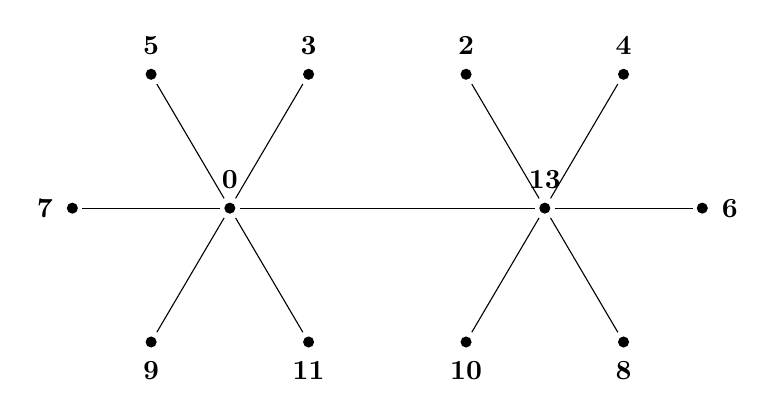
\begin{tikzpicture}
		
		\node[label=above:$\bf{0}$] (v1) at ( 0.0,   0) {};\fill (v1) circle (2pt);
		\node[label=above:$\bf{3}$] (v2) at ( 1.0, 1.7) {};\fill (v2) circle (2pt);
		\node[label=above:$\bf{5}$] (v3) at (-1.0, 1.7) {};\fill (v3) circle (2pt);
		\node[label=left:$\bf{7}$] (v4) at (-2.0,   0) {};\fill (v4) circle (2pt);
		\node[label=below:$\bf{9}$] (v5) at (-1.0,-1.7) {};\fill (v5) circle (2pt);
		\node[label=below:$\bf{11}$] (v6) at ( 1.0,-1.7) {};\fill (v6) circle (2pt);
		
		\node[label=above:$\bf{13}$] (v7) at ( 4.0,-  0) {};\fill (v7) circle (2pt);
		\node[label=above:$\bf{2}$] (v8) at ( 3.0, 1.7) {};\fill (v8) circle (2pt);
		\node[label=above:$\bf{4}$] (v9) at ( 5.0, 1.7) {};\fill (v9) circle (2pt);
		\node[label=right:$\bf{6}$] (v10) at ( 6.0, 0) {};\fill (v10) circle (2pt);
		\node[label=below:$\bf{8}$] (v11) at ( 5.0,-1.7) {};\fill (v11) circle (2pt);
		\node[label=below:$\bf{10}$] (v12) at ( 3.0,-1.7) {};\fill (v12) circle (2pt);
		
		
		\draw[-] (v1) to (v2);
		\draw[-] (v1) to (v3);
		\draw[-] (v1) to (v4);
		\draw[-] (v1) to (v5);
		\draw[-] (v1) to (v6);

		\draw[-] (v1) to (v7);

		\draw[-] (v7) to (v8);
		\draw[-] (v7) to (v9);
		\draw[-] (v7) to (v10);
		\draw[-] (v7) to (v11);
		\draw[-] (v7) to (v12);		
		
	\end{tikzpicture}
	}
\caption{$L(3,2,1)$}
\label{}
\end{figure}

% Fig 3
\begin{figure}[hb]
\centering

	\vbox{ 
		\begin{tikzpicture}
		
		\node[label=left:$\bf{2}$] (v1) at ( 0.0, 0.0) {};\fill (v1) circle (2pt);
		\node[label=above:$\bf{0}$] (v2) at ( 1.0, 1.7) {};\fill (v2) circle (2pt);
		\node[label=above:$\bf{3}$] (v3) at ( 3.0, 1.7) {};\fill (v3) circle (2pt);
		\node[label=right:$\bf{5}$] (v4) at ( 4.0, 0.0) {};\fill (v4) circle (2pt);	
		\node[label=below:$\bf{1}$] (v5) at ( 3.0,-1.7) {};\fill (v5) circle (2pt);
		\node[label=below:$\bf{4}$] (v6) at ( 1.0,-1.7) {};\fill (v6) circle (2pt);

		\draw[-] (v1) to (v2); \draw[-]  (v1) to (v6);
		\draw[-] (v2) to (v3); \draw[-]  (v2) to (v6);
		\draw[-] (v3) to (v4); \draw[-]  (v3) to (v5);
		\draw[-] (v4) to (v5);
		\draw[-] (v5) to (v6);

	\end{tikzpicture}
	}
\caption{$L(2,1)$}
\label{}
\end{figure}

% Fig 4
\begin{figure}[hb]
\centering

	\vbox{ 
		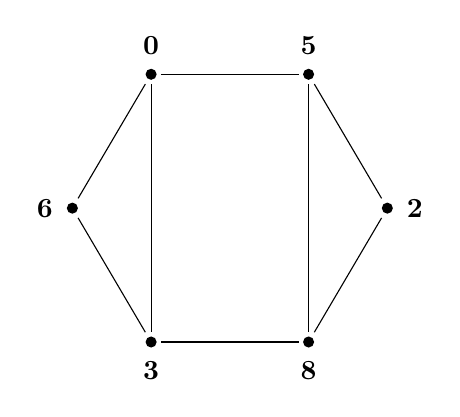
\begin{tikzpicture}
		
		\node[label=left:$\bf{6}$] (v1) at ( 0.0, 0.0) {};\fill (v1) circle (2pt);
		\node[label=above:$\bf{0}$] (v2) at ( 1.0, 1.7) {};\fill (v2) circle (2pt);
		\node[label=above:$\bf{5}$] (v3) at ( 3.0, 1.7) {};\fill (v3) circle (2pt);
		\node[label=right:$\bf{2}$] (v4) at ( 4.0, 0.0) {};\fill (v4) circle (2pt);	
		\node[label=below:$\bf{8}$] (v5) at ( 3.0,-1.7) {};\fill (v5) circle (2pt);
		\node[label=below:$\bf{3}$] (v6) at ( 1.0,-1.7) {};\fill (v6) circle (2pt);

		\draw[-] (v1) to (v2); \draw[-]  (v1) to (v6);
		\draw[-] (v2) to (v3); \draw[-]  (v2) to (v6);
		\draw[-] (v3) to (v4); \draw[-]  (v3) to (v5);
		\draw[-] (v4) to (v5);
		\draw[-] (v5) to (v6);
		
	\end{tikzpicture}
	}
\caption{}
\label{}
\end{figure}

% Fig 5
\begin{figure}[hb]
\centering

	\vbox{ 
		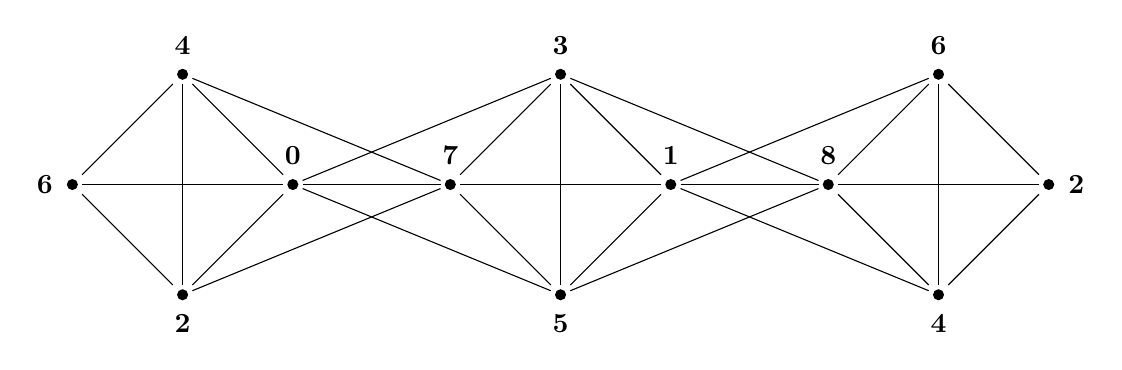
\begin{tikzpicture}

		\node[label=left: $\bf{ 6}$] (v1) at ( 0.0, 0.0) {};\fill (v1) circle (2pt);
		\node[label=above:$\bf{ 4}$] (v2) at ( 1.4, 1.4) {};\fill (v2) circle (2pt);
		\node[label=above:$\bf{ 0}$] (v3) at ( 2.8, 0.0) {};\fill (v3) circle (2pt);
		\node[label=below:$\bf{ 2}$] (v4) at ( 1.4,-1.4) {};\fill (v4) circle (2pt);
		
		\node[label=above:$\bf{ 7}$] (v5) at ( 4.8, 0.0) {};\fill (v5) circle (2pt);
		\node[label=above:$\bf{ 3}$] (v6) at ( 6.2, 1.4) {};\fill (v6) circle (2pt);
		\node[label=above:$\bf{ 1}$] (v7) at ( 7.6, 0.0) {};\fill (v7) circle (2pt);
		\node[label=below:$\bf{ 5}$] (v8) at ( 6.2,-1.4) {};\fill (v8) circle (2pt);
	
		\node[label=above:$\bf{ 8}$] (v9)  at ( 9.6, 0.0) {};\fill (v9) circle (2pt);
		\node[label=above:$\bf{ 6}$] (v10) at ( 11.0, 1.4) {};\fill (v10) circle (2pt);
		\node[label=right:$\bf{ 2}$] (v11) at (12.4, 0.0) {};\fill (v11) circle (2pt);
		\node[label=below:$\bf{ 4}$] (v12) at ( 11.0,-1.4) {};\fill (v12) circle (2pt);

		\draw[-] (v1) to (v2); \draw[-]  (v1) to (v3); \draw[-]  (v1) to (v4);
		\draw[-] (v2) to (v3); \draw[-]  (v2) to (v4);
		\draw[-] (v3) to (v4);
		
		\draw[-] (v2) to (v5);
		\draw[-] (v3) to (v5);		
		\draw[-] (v4) to (v5);
		
    	\draw[-] (v6) to (v3);
		\draw[-] (v5) to (v3);		
		\draw[-] (v8) to (v3);
				
		\draw[-] (v5) to (v6); \draw[-]  (v5) to (v7); \draw[-]  (v5) to (v8);
		\draw[-] (v6) to (v7); \draw[-]  (v6) to (v8);
		\draw[-] (v7) to (v8);

		\draw[-] (v6) to (v9);
		\draw[-] (v7) to (v9);		
		\draw[-] (v8) to (v9);
		
    	\draw[-] (v10) to (v7);
		\draw[-] (v9) to (v7);		
		\draw[-] (v12) to (v7);
		
		\draw[-] (v9) to (v10); \draw[-] (v9) to (v11); \draw[-] (v9) to (v12);
		\draw[-] (v10) to (v11); \draw[-]  (v10) to (v12);
		\draw[-] (v11) to (v12);
		
	\end{tikzpicture}
	}
\caption{$L(2,1)$}
\label{}
\end{figure}

% Fig 6
\begin{figure}[hb]
\centering

	\vbox{ 
		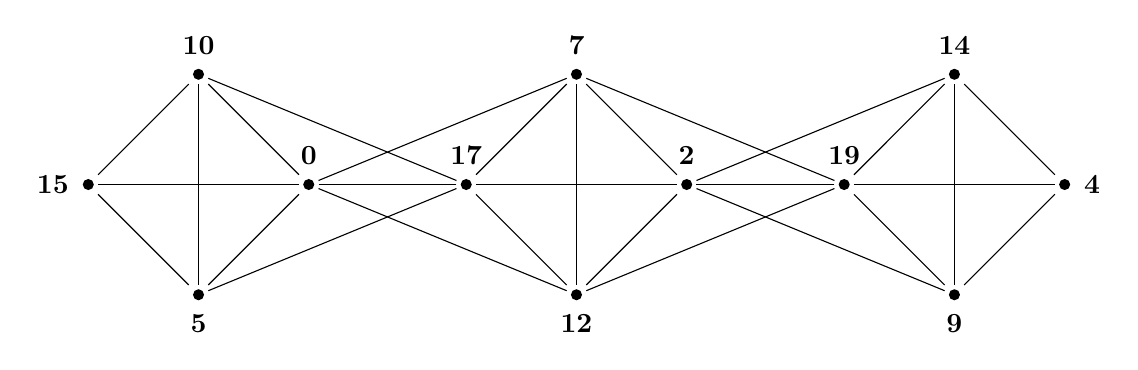
\begin{tikzpicture}
		
		\node[label=left:$\bf{15}$] (v1) at ( 0.0, 0.0) {};\fill (v1) circle (2pt);
		\node[label=above:$\bf{10}$] (v2) at ( 1.4, 1.4) {};\fill (v2) circle (2pt);
		\node[label=above:$\bf{ 0}$] (v3) at ( 2.8, 0.0) {};\fill (v3) circle (2pt);
		\node[label=below:$\bf{ 5}$] (v4) at ( 1.4,-1.4) {};\fill (v4) circle (2pt);
		
		\node[label=above:$\bf{17}$] (v5) at ( 4.8, 0.0) {};\fill (v5) circle (2pt);
		\node[label=above:$\bf{ 7}$] (v6) at ( 6.2, 1.4) {};\fill (v6) circle (2pt);
		\node[label=above:$\bf{ 2}$] (v7) at ( 7.6, 0.0) {};\fill (v7) circle (2pt);
		\node[label=below:$\bf{12}$] (v8) at ( 6.2,-1.4) {};\fill (v8) circle (2pt);
	
		\node[label=above:$\bf{19}$] (v9)  at ( 9.6, 0.0) {};\fill (v9) circle (2pt);
		\node[label=above:$\bf{14}$] (v10) at (11.0, 1.4) {};\fill (v10) circle (2pt);
		\node[label=right:$\bf{ 4}$] (v11) at (12.4, 0.0) {};\fill (v11) circle (2pt);
		\node[label=below:$\bf{ 9}$] (v12) at (11.0,-1.4) {};\fill (v12) circle (2pt);

		\draw[-] (v1) to (v2); \draw[-]  (v1) to (v3); \draw[-]  (v1) to (v4);
		\draw[-] (v2) to (v3); \draw[-]  (v2) to (v4);
		\draw[-] (v3) to (v4);
		
		\draw[-] (v2) to (v5);
		\draw[-] (v3) to (v5);		
		\draw[-] (v4) to (v5);
		
    	\draw[-] (v6) to (v3);
		\draw[-] (v5) to (v3);		
		\draw[-] (v8) to (v3);
				
		\draw[-] (v5) to (v6); \draw[-]  (v5) to (v7); \draw[-]  (v5) to (v8);
		\draw[-] (v6) to (v7); \draw[-]  (v6) to (v8);
		\draw[-] (v7) to (v8);

		\draw[-] (v6) to (v9);
		\draw[-] (v7) to (v9);		
		\draw[-] (v8) to (v9);
		
    	\draw[-] (v10) to (v7);
		\draw[-] (v9) to (v7);		
		\draw[-] (v12) to (v7);
		
		\draw[-] (v9) to (v10); \draw[-] (v9) to (v11); \draw[-] (v9) to (v12);
		\draw[-] (v10) to (v11); \draw[-]  (v10) to (v12);
		\draw[-] (v11) to (v12);
		
	\end{tikzpicture}
	}
\caption{$L(3,2,1)$}
\label{}
\end{figure}

% Fig 7
\begin{figure}[hb]
\centering

	\vbox{ 
		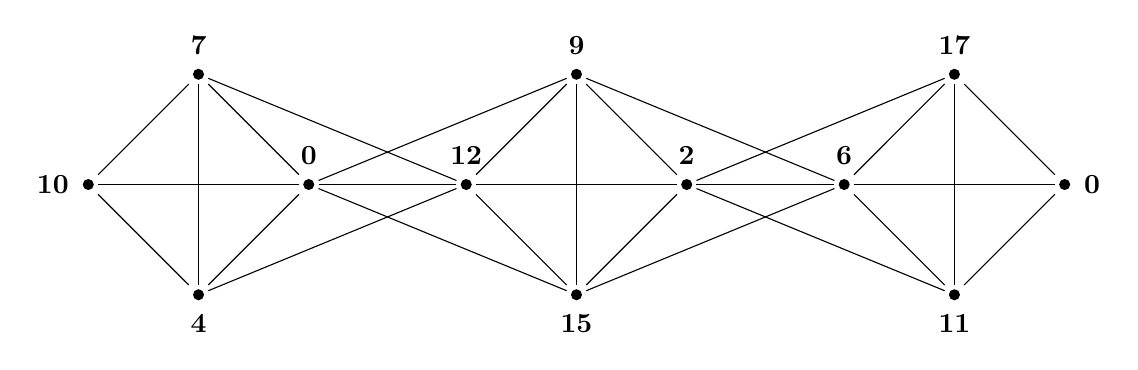
\begin{tikzpicture}
		
		\node[label=left: $\bf{10}$] (v1) at ( 0.0, 0.0) {};\fill (v1) circle (2pt);
		\node[label=above:$\bf{ 7}$] (v2) at ( 1.4, 1.4) {};\fill (v2) circle (2pt);
		\node[label=above:$\bf{ 0}$] (v3) at ( 2.8, 0.0) {};\fill (v3) circle (2pt);
		\node[label=below:$\bf{ 4}$] (v4) at ( 1.4,-1.4) {};\fill (v4) circle (2pt);
		
		\node[label=above:$\bf{12}$] (v5) at ( 4.8, 0.0) {};\fill (v5) circle (2pt);
		\node[label=above:$\bf{ 9}$] (v6) at ( 6.2, 1.4) {};\fill (v6) circle (2pt);
		\node[label=above:$\bf{ 2}$] (v7) at ( 7.6, 0.0) {};\fill (v7) circle (2pt);
		\node[label=below:$\bf{15}$] (v8) at ( 6.2,-1.4) {};\fill (v8) circle (2pt);
	
		\node[label=above:$\bf{ 6}$] (v9)  at ( 9.6, 0.0) {};\fill (v9) circle (2pt);
		\node[label=above:$\bf{17}$] (v10) at (11.0, 1.4) {};\fill (v10) circle (2pt);
		\node[label=right:$\bf{ 0}$] (v11) at (12.4, 0.0) {};\fill (v11) circle (2pt);
		\node[label=below:$\bf{11}$] (v12) at (11.0,-1.4) {};\fill (v12) circle (2pt);

		\draw[-] (v1) to (v2); \draw[-]  (v1) to (v3); \draw[-]  (v1) to (v4);
		\draw[-] (v2) to (v3); \draw[-]  (v2) to (v4);
		\draw[-] (v3) to (v4);
		
		\draw[-] (v2) to (v5);
		\draw[-] (v3) to (v5);		
		\draw[-] (v4) to (v5);
		
    	\draw[-] (v6) to (v3);
		\draw[-] (v5) to (v3);		
		\draw[-] (v8) to (v3);
				
		\draw[-] (v5) to (v6); \draw[-]  (v5) to (v7); \draw[-]  (v5) to (v8);
		\draw[-] (v6) to (v7); \draw[-]  (v6) to (v8);
		\draw[-] (v7) to (v8);

		\draw[-] (v6) to (v9);
		\draw[-] (v7) to (v9);		
		\draw[-] (v8) to (v9);
		
    	\draw[-] (v10) to (v7);
		\draw[-] (v9) to (v7);		
		\draw[-] (v12) to (v7);
		
		\draw[-] (v9) to (v10); \draw[-] (v9) to (v11); \draw[-] (v9) to (v12);
		\draw[-] (v10) to (v11); \draw[-]  (v10) to (v12);
		\draw[-] (v11) to (v12);
		
	\end{tikzpicture}
	}
\caption{$L(3,2,1)$}
\label{}
\end{figure}

\end{document}



 
